\subsection{Robot Operating System}
The Robot Operating System (ROS) was developed by Willow Garage,  originally
for  the  PR2  robot  in  2007  [Quigley et al., 2009].   It  is  an  open  source  framework
for  developing  software  in  robotics  with  a  focus  on  the  ability  to  run  parallel  on
distributed  computer  systems.   It  can  be  run  on  different  operating  systems,  but
only Ubuntu and Debian are officially supported.  Its main advantage is a big library
of  available  software  modules  for  common  robotics  tasks.   These  are  developed,
maintained and documented by the ROS community and adding further modules is
easy.  Using ROS decreases the time for developing software as most of the parts can
be taken from the library.  In the following section, a short overview of the concepts
of ROS is provided.  A deeper insight can be found in the online documentation [3].

\subsubsection*{Nodes}
A node is a process in the ROS system.  It can communicate with other ROS nodes
via  topics  or  services.   In  doing  so,  all  nodes  form  a  computational  graph.   Each
node has typically a clearly defined subtask.  For example one node gets the camera
image, a second node detects balls on this image, and a third node computes the
ball positions.  Nodes can be easily reused in different tasks, for example the node
which gets the camera image can be reused in a different task that detects goals.
Open  source  implementations  of  nodes  for  most  standard  subtasks,  especially
hardware controlling, already exist.  Thereby the effort in implementing a new task
is drastically decreased.  The most important packages used for this thesis are men-
tioned in section 2.3.7

\begin{figure}[htbp]
	\centering	    
	\begin{tikzpicture}[shorten > = 1pt]
		% Place nodes
		\node [node] (image_provider) {image\_provider};
		\node [topic, below of=image_provider] (/image) {/image\\sensor\_msgs/Image.msg};
		\node [node, below left of=/image] (line_detection) {line\_detection};
		\node [node, below right of=/image] (stop_detection) {stop\_detection};
		\node [topic, below of=line_detection,xshift=-0.5cm] (/line) {/line\\example\_msgs/Line.msg};
		\node [topic, below of=stop_detection,xshift=0.5cm] (/stop) {/stop\\example\_msgs/Stop.msg};
		\node [node, below of=/image, yshift=-3.0cm] (navigation) {navigation};
		\node [topic, below of=navigation] (/cmd_vel) {/cmd\_vel\\geometry\_msgs/Twist.msg};
		\node [node, below of=/cmd_vel,yshift=1cm] (robot_control) {robot\_control};
		% % Draw edges
		\path [line] (image_provider) -- (/image);
		\path [line] (/image) -- (line_detection);
		\path [line] (/image) -- (stop_detection);
		\path [line] (line_detection) -- (/line);
		\path [line] (stop_detection) -- (/stop);
		\path [line] (/line) -- (navigation);
		\path [line] (/stop) -- (navigation);
		\path [line] (navigation) -- (/cmd_vel);
		\path [line] (/cmd_vel) -- (robot_control);
	\end{tikzpicture}
	\caption{ตัวอย่างสถาปัตยกรรมของ ROS}
	\label{fig:poppy_humanoidz}
\end{figure}

Example ROS architecture for a simple wheeled robot with the task to
follow  a  line  until  it  finds  a  stop  marker.   The  nodes  are  displayed  as
ellipses with a name and the topics are shown as rectangles with name
and message type.  First, an image is provided from the camera.  Lines
and stop markers are detected on this image.  Based on this information,
a navigation node computes the necessary movement of the robot and
publishes it.  The robot
control node is then controlling the motors of
the robot accordingly



\begin{table}[htbp]
	\begin{subtable}[h]{0.40\textwidth}
		\centering
		\begin{tabular}{| p{4cm}| p{1.5cm} |}
			\hline 
			\multicolumn{2}{|c|}{Twist.msg} \\
			\hline
			geometry\_msgs/Vector3 & linear  \\
			geometry\_msgs/Vector3 & angular \\
			\hline  
		\end{tabular}
		\caption{First Week}
		\label{tab:week1}
	\end{subtable}
	\hfill
	\begin{subtable}[h]{0.40\textwidth}
		\centering
		\begin{tabular}{| p{1.5cm}| p{2.5cm} |}
			\hline 
			\multicolumn{2}{|c|}{Stop.msg} \\
			\hline
			uint8   & RED = 0   \\
			uint8   & GREEN = 1 \\
			uint8   & color     \\
			float32 & distance  \\
			\hline  
		\end{tabular}
		\caption{First Week}
		\label{tab:week1}
	\end{subtable}
	\caption{Max and min temps recorded in the first two weeks of July}
	\label{tab:temps}
\end{table}

two example messages.  The
Twist
message (left) is already defined in
ROS. The
Stop
message (right) is newly defined for the special applica-
tion case of figure 2.4.

\subsubsection*{Topics and Messages}
Messages are the main communication method between ROS nodes.  Messages are
always published on a topic, which is identified by a name and can only transmit
one  type  of  message.   A  node  can  subscribe  to  a  topic  and  will  get  the  messages
other nodes publish to it.  Each node can subscribe to and publish on any number
of topics and will not know with whom it communicates.
Communication can happen between nodes running on the same computer as well
as nodes distributed over different computers,  as long as they are connected with
an TCP/IP network.  This is not only useful for parallelization but also eases the
visualization of the robots state on a separate desktop computer.  Each message has
a type which is either predefined in the ROS system or defined by a user package.
The interface of a node is mainly defined by the types of the messages it subscribes
and publishes.  These types can be either predefined in ROS or be newly created by
a developer, cp.  figure 2.5.

\subsubsection*{roscore}
The
roscore
is the most central part of a running ROS system.  It consists of the
rosmaster
,  the  ROS  parameter  server  and  the
rosout
logging  node.   The  ROS
master is registering which topics are published by the nodes and on which topics
nodes want to subscribe.  If one node wants to subscribe to a topic which another
node is publishing,  a peer-to-peer connection is established from one node to the
other.  Thereby the master does not become a bottleneck since it only connects the
nodes but does not need to handle the messages.  To do this, a subscribing node asks
the master for a list of nodes which publish on this named topic.  The master holds
a  table  of  all  publishers  and  sends  their  names  to  the  subscribing  nodes.   It  also
remembers which nodes are subscribing to this topic, if a new publisher is started
later.  This process is shown in figure 2.6.
The ROS parameter server is a global key-value store.  It is mainly designed to
be  used  for  static  configuration  parameters.   Transmission  of  data  between  nodes
should be done via topics to prevent making the parameter server a bottleneck.  All
parameters are globally visible.  If a parameter should be able to be changed during
runtime,  dynamic reconfigure can be used.  It provides the possibility to state on
compile  time  which  parameter  values  should  be  changeable  and  provides  an
rqt
plug-in for it, see section 2.3.9.  The
rosout
logging node subscribes to the
/rosout
topic which is the standard topic for logging.  ROS has built in methods to send
data to this topic which are displayed on runtime and written in a log file

\subsubsection*{Services}
Services  can  be  seen  as  remote  procedure  calls  (RPC).  In  contrast  to  messages
which are an unidirectional stream of data,  service calls are blocking and waiting
for a response.  They have defined types which consist of a request and a response
message.  The node providing the service is called server and the node calling the
service  is  called  client.   Services  are  useful  for  fast  tasks,  but  should  not  be  used
when getting the result can take a long time,  because the calling node is blocked
until completion.  For longer tasks, actions should be used (section 2.3.5).  A possible
service for the example described in figure 2.4 would be a manual stop service.  It
would be advertised by the navigation node and would stop the robot even without
markers.  As this would take not a lot of time, basically just alternating the state of
the navigation node, this would be possible to do with a blocking service call.

\subsubsection*{Actions}
Actions  are  used  when  a  task  which  takes  a  long  time  should  be  called  asyn-
chronously, in contrast to the synchronous service calls.  Each action has a specified
type which consists of three messages:  goal, feedback, and result.  A node providing
the action, the action server, is called by another node, the action client, by sending
a goal.  The action server will now try to achieve this goal, while the action client is
not blocked and can perform other tasks.  The server will constantly send feedback
messages to the client to inform it about the status of the process towards the goal.
The server will send a result message when the goal was reached or if the action was
interrupted.  Actions can be interrupted by sending new goals which the server con-
siders more important or by request of the action client, for example, if the sent goal
is not useful anymore.  A possible action for the example described in 2.4 would be
driving a certain distance on the line.  This needs some time because the robot has
to move.  Therefore a blocking call is not feasible.  The action runs asynchronously
and can also be interrupted, for example, if the line ends before reaching the desired
distance.

\subsubsection*{Code Organization}
The smallest and main unit for organizing software for ROS is a package.  A package
has a
package.xml
\ref{fig:example_packagexml} which describes different metadata of this package,
e.g.  the package name, the author, the license and dependencies on other packages.
A package can build on its own if all dependencies are met.  The content can, among
other things, be ROS nodes, visualization plug ins, libraries or datasets.  It can be
distinguished between dependencies on build and runtime.  Different packages can
be grouped in meta-packages, which hold no content of their own but only collect
packages which belong together.

\begin{figure}[htbp]
    \centering
    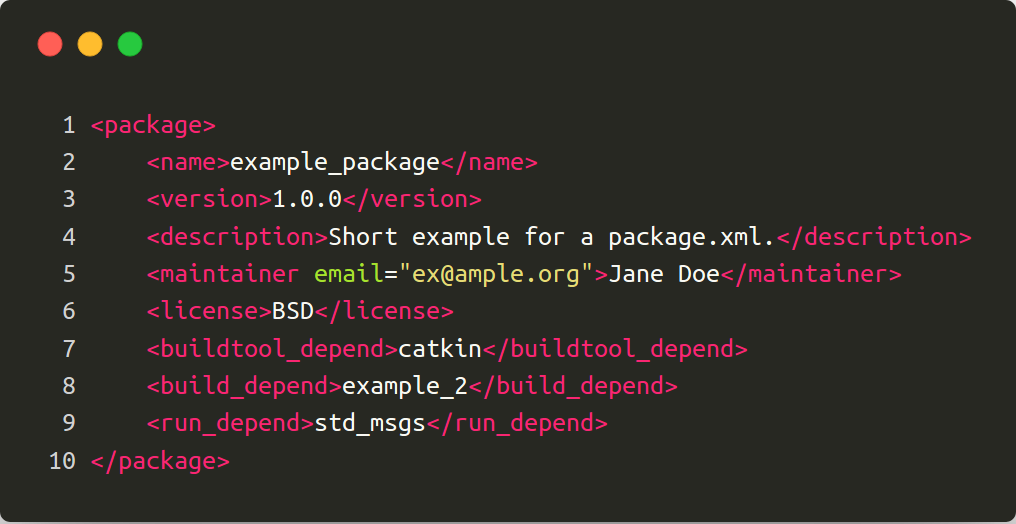
\includegraphics[width=0.8\textwidth]{chapter2/images/example_packagexml.png}
	\caption{ตัวอย่างไฟล์ package.xml แต่ละ tags สามารถใช้ในการบอกข้อมูลของ package นี้
	ใครเป็นเจ้าของ ใครเป็นคนเขียน รวมไปถึง dependencies ที่จำเป็นต้องใช้ของ package นี้ด้วย}
    \label{fig:example_packagexml}
\end{figure}

\subsubsection*{Code Distribution}
การที่จะนำ Nodes กลับมาใช้ใหม่หรือเอาออกมาแชร์ได้นั้น จะต้องมีการทำเอกสารของ Packages นั้นๆด้วย
โดยปกติแล้วจะถูกนำไปเก็บไว้ที่ GitHub และ package dependencies จะบอกไว้ในไฟล์ package.xml
เรียบร้อยแล้ว เพื่อให้ง่ายต่อการนำไปติดตั้ง หากผู้ที่นำไปใช้พัฒนาต่อหรือแก้ไขข้อผิดพลาดก็สามารถที่จะช่วยกันได้
โดยการ Pull request หรือ Report issues ได้

\subsubsection*{ROS Packages ที่ใช้ในงานวิจัย}
ในส่วนนี้จะอธิบายคร่าวๆถึง ROS standard packages ที่จะเอามาใช้ในงานวิจัยครั้งนี้
\paragraph*{rosbag}
rosbag เป็นแพกเกจที่สามารถบันทึก message ที่ส่งหากันในระหว่างที่ ROS กำลังทำงานได้
ไฟล์ที่บันทึกจะเรียกว่า rosbag ประโยชน์ของมันคือเราสามารถเอาเข้ามาใช้ในการตรวจสอบ
หรือนำมาเล่นซ้ำได้ อีกทั้งยังง่ายต่อการค้นหาข้อผิดพลาดอีกด้วย

\paragraph*{tf2}
tf2 เป็นแพกเกจที่สามารถติดตามการเปลี่ยนแปลงของ Coordinate frame เราสามารถใช้ในการหาความสัมพันธ์ระหว่าง
frame ได้ ยกตัวอย่างเช่นหากเราต้องการหาตำแหน่งของ foot เทียบกับ pelvis ก็สามารถใช้ tf2 หาได้

robot\_state\_publisher แพกเกจที่ subscribe JointState message เพื่อที่จะนำตำแหน่งของของข้อต่อ
และแปลงให้อยู่ในรูปข้อมูลของ tf2, tf2 สามารถเรียกจาก Node ใดๆก็ได้เพื่อที่จะหา Coordinate frame ที่ต้องการได้

\paragraph*{URDF}
Unified Robot Description Format (URDF) เป็นไฟล์ XML ที่เอาไว้อธิบายลักษณะของหุ่นยนต์
ใน ROS มีแพกเกจที่ใช้สำหรับการอ่านไฟล์ คือ urdf\_parser แต่ไฟล์นี้ก็มีการใช้งานโดย tf2 เช่นกัน

\paragraph*{xacro}
xacro เป็นไฟล์ XML เช่นเดียวกับ URDF โดยไฟล์ xacro นี้มีประโยชน์มากในการใช้งานใน ROS เพราะว่าทำให้การเขียนไฟล์
URDF ง่ายขึ้น เพราะสามารถทำเป็นมาโครได้ สามารถปรับแต่งค่าตัวแปรต่างๆได้ง่ายขึ้น

\subsubsection*{Visualization}
One of ROS’ core strengths is providing different tools for visualization.  Due to its
publisher-subscriber architecture, it is very easy to establish a data stream from the
program to the visualization.  Either the visualization can subscribe on topics that
are already being in use or additional topics can be provided from the software to
deliver more information to the visualization.  Messages in ROS are only published
if there is a subscriber on the topic, therefore publishing additional topics for visu-
alization reasons does not cost performance when the visualization is not running.
ROS provides two main tools for visualization which can be extended by plug-ins.
It is also possible to implement own tools which are independent from these.

\paragraph*{rqt}
rqt  is  a  QT  based  interface  with  ROS  connection \ref{fig:ros_gui_example}   Plug-ins  can  be
launched and provide a
QtWidget
.  Multiple widgets can be displayed at the same
time.  They can be resized and positioned by drag and drop.  ROS provides a set
of plug-ins but writing an own plug-in is possible too.  These plug-ins can be used
to visualize data in 2D but also to provide a controlling interface.  In the following,
some examples of important plug-ins are shown.
The
node
graph
plug-in shows all currently running nodes and topics.  Published
and subscribed topics are connected to their nodes and thereby it is easy to see the
flow of data.  This plug-in is especially helpful to get an overview of the running
software and to find misconnected nodes.
The
topic
monitor
lists all current topics.  It is possible to subscribe to them and
to get the current transmitted values.  Further on, statistics about the publishing
rate and the used bandwidth can be shown for each topic.
The
rqt
plot
plug-in  enables  live  plotting  of  data,  using
matplotlib
.    The
dynamic
reconfigure
plug-in provides an interface to change parameter values pre-
viously defined to be reconfigurable.  This is useful when tuning parameter values,
because  changing  it  is  possible  on  the  fly  and  does  not  require  a  restart  of  the
software


\begin{figure}[htbp]
    \centering
    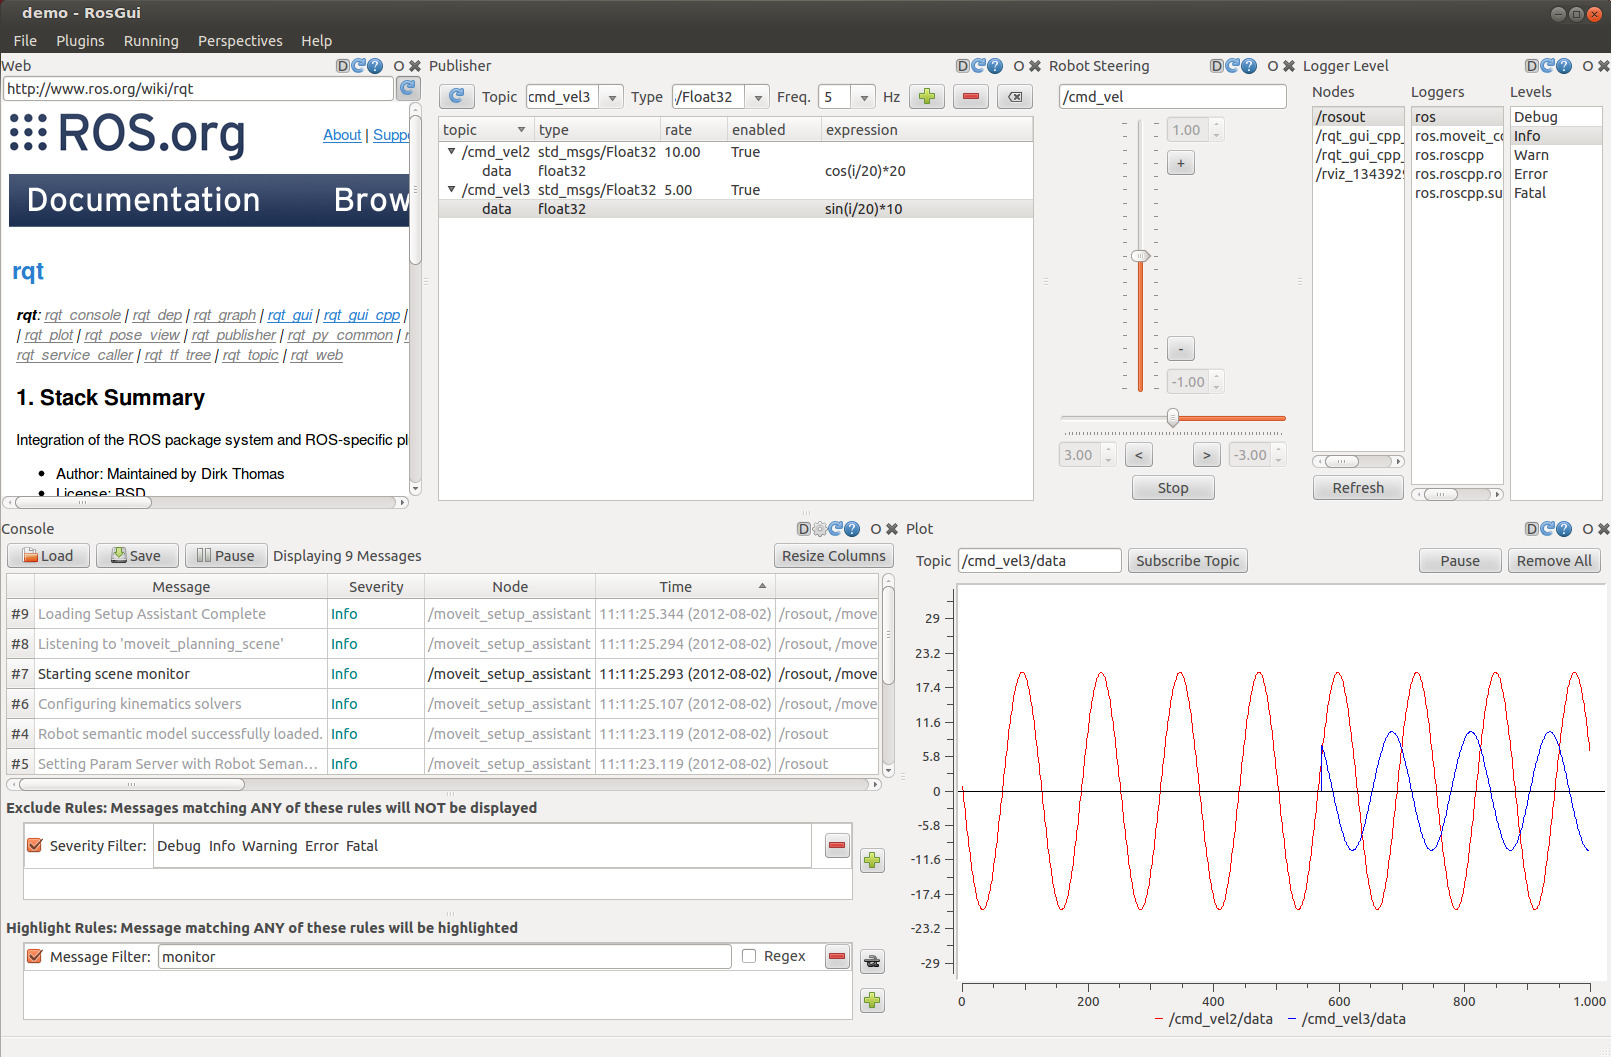
\includegraphics[width=0.8\textwidth]{chapter2/images/ros_gui_example.png}
	\caption{ตัวอย่างการแสดงผลใน rqt ในรูปเป็นการนำ rqt มาเขียนเป็น GUI ให้ผู้ใช้สามารถใช้งานได้ง่าย
	และสามารถที่จะปรับแต่ง parameters ต่างๆได้เรียลไทม์}
    \label{fig:ros_gui_example}
\end{figure}

\paragraph*{RViz}
RViz  provides  a  3D  visualization  of  the  robots  state  and  its  environment.   The
standardized URDF format is used to get a visual robot model, which is then used
to  show  the  current  positions  of  the  robots  joints.   Furthermore,  sensor  data  can
be displayed using marker messages.  These messages can be published by any node
and define three dimensional states which are displayed in RViz.  This is for example
helpful to get a visualization of recognized objects.  Furthermore, a lot of different
standard  ROS  messages  can  directly  be  visualized  in  RViz,  e.g.   camera  images,
depth  clouds,  laser  scans  and  point  clouds.   Thereby  RViz  provides  visualization
without additional effort, if the standard messages are used.  It is especially used for
localization and mapping, because it is possible to see the current sensor inputs of
the robot as well as its map in the same window \ref{fig:example_visualization_rviz}

\begin{figure}[htbp]
    \centering
    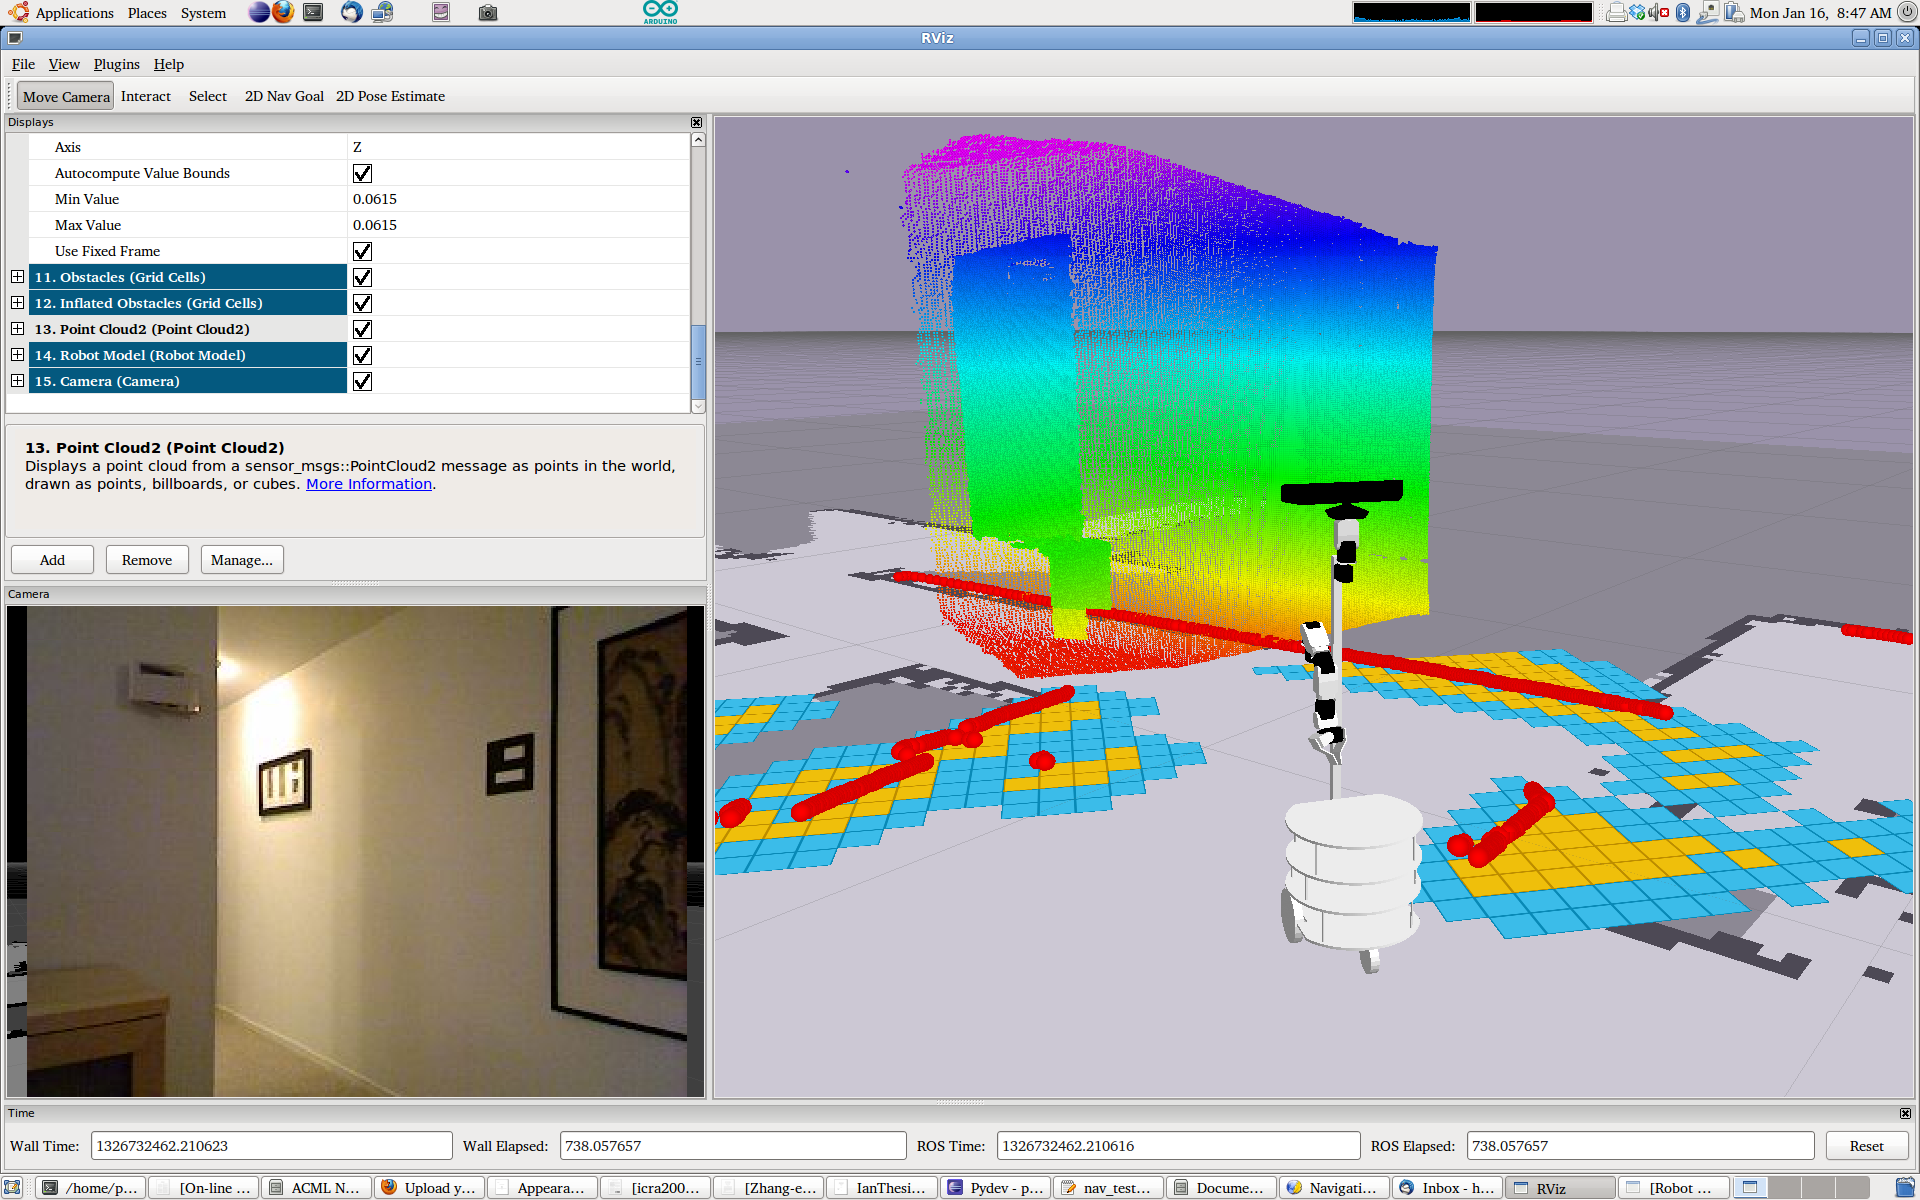
\includegraphics[width=0.8\textwidth]{chapter2/images/nav_test_rviz_2.png}
	\caption{ตัวอย่างการแสดงผลใน RViz ในรูปนี้เป็นเคสของหุ่นยนต์เคลื่อนที่ด้วยล้อ และทำแผนที่ด้วยข้อมูลความลึกที่ได้มาจาก Kinect}
    \label{fig:example_visualization_rviz}
\end{figure}



\subsubsection*{Simulation}
Simulation is a crucial part when developing robot software, since it gives the devel-
oper the possibility to run his software without using hardware.  This can prevent
hardware damages because bugs can be found before running it on the robot and
it can be used to accelerate development, e.g.  by testing in faster than real time.
While ROS can generally use any simulator, Gazebo is normally preferred, since it
has a good ROS integration and was also originally developed for ROS. In order to
use Gazebo, an URDF of the robot is required.
This  URDF  is  used  to  display  the  robot  in  the  simulator  and  to  compute  its
collisions with itself and the environment.  The simulator can provide sensor data
in  the  corresponding  standard  messages.   To  actuate  the  servos  of  the  robot,  dif-
ferent  controllers  are  available  which  work  with  the  corresponding  messages,  e.g.
JointTrajectory
